
\documentclass[12pt]{article}
\usepackage[margin=1in]{geometry}
\bibliographystyle{plainnat}
\usepackage[slantedGreek]{mathpazo}
\usepackage[pdftex]{graphicx}
\usepackage{amsfonts}
\usepackage{amssymb}
\usepackage{float}
\usepackage{amsmath}%
\usepackage{hyperref}
\usepackage{natbib}
\usepackage{color}
\usepackage{algorithm}
\usepackage[noend]{algpseudocode}
\setlength{\emergencystretch}{2em}

\title{Generative Bayesian Hyperparameter Tuning}
\author{	
	\makebox[.4\linewidth]{Hedibert Lopes}\\\textit{Insper}\\\and
	\makebox[.4\linewidth]{Nick Polson}\\\textit{Chicago Booth}\\\textit{University of Chicago}\\\and
	\makebox[.4\linewidth]{Vadim Sokolov\footnote{Hedibert Lopes is Professor of Statistics and Econometrics at Insper: hlopes@insper.edu.br. Nick Polson is Professor of Econometrics and Statistics at Chicago Booth, University of Chicago: ngp@chicagobooth.edu. Vadim Sokolov is Associate Professor at Volgenau School of Engineering, George Mason University: vsokolov@gmu.edu.}}\\\textit{Department of Systems Engineering}\\\textit{and Operations Research}\\\textit{George Mason University}
}

\date{First Version: 20 January 2025\\This Version: \today}

\graphicspath{{./fig/}}

\begin{document}

\maketitle
\begin{abstract}
\noindent Choosing regularization hyper-parameters is a core task in statistical and machine-learning practice. Standard approaches include cross-validation, which is computationally expensive because the model must be retrained for every candidate value, and marginal-likelihood methods, which provide analytic tuning criteria but are limited to specific model classes. We develop a generative approach to hyper-parameter tuning that combines two ideas: the weighted Bayesian bootstrap (WBB), which converts fast optimization into approximate posterior draws by randomly reweighting the training objective, and neural-network-based amortization, which learns a transport map (generator) from hyper-parameters and bootstrap weights to the corresponding fitted model. Once trained, the generator produces fitted parameters for any new hyper-parameter value via a single forward pass, replacing the expensive retraining loop. We show how this viewpoint connects to classical generalized cross-validation and the generative multi-purpose sampler, and we note how auxiliary-variable representations can extend the same template to non-Gaussian losses such as quantile regression.
\end{abstract}

\noindent\textit{Keywords:} Amortized inference; Bayesian bootstrap; Cross-validation; Hyperparameter optimization; Transport map; Weighted $M$-estimation.

\section{Introduction}

Hyper-parameters such as regularization strengths, robustness or quantile levels, and architectural or optimization settings have an outsized impact on predictive performance and calibration. Several families of methods exist for choosing these hyper-parameters, each with characteristic trade-offs.

Cross-validation (CV) is the most widely used approach: the data are split into training and validation folds, the model is retrained for each candidate hyper-parameter value, and the value that minimizes validation error is selected \citep{stone1974crossvalidatory}. CV is general-purpose but computationally expensive, since the full training procedure must be repeated for every candidate value and every fold.

Marginal-likelihood and empirical Bayes methods avoid repeated retraining by deriving analytic tuning criteria \citep{berger1985statistical}. Generalized cross-validation (GCV) is a classical example: for linear smoothers such as ridge regression, the leave-one-out prediction error can be estimated from a single fit using the trace of the hat matrix \citep{golub1979generalized}. These methods are fast but restricted to model classes where the optimizer and the tuning criterion admit closed-form expressions \citep{golub1979generalized}.

Bayesian approaches place a prior on the hyper-parameter and compute or approximate the posterior, providing a principled framework for model comparison. In practice, however, posterior computation typically requires MCMC over the joint space of parameters and hyper-parameters, which is expensive when the model is large or when the conditional distributions mix slowly \citep{gamerman2006markov}. Variational approximations offer an alternative but require careful design of the variational family \citep{blei2017variational}. A concrete example is estimating the degrees-of-freedom parameter $\nu$ of a Student-$t$ distribution: the profile likelihood is flat in $\nu$, improper priors lead to improper posteriors, and MCMC mixes slowly because the marginal likelihood $p(y\mid\nu)$ is nonlinear in $\nu$ \citep{fonseca2008objective}.

This paper develops a generative approach to hyper-parameter tuning that combines two ideas \citep{nareklishvili2024generative,polson2025generative,nareklishvili2023generative}. First, the weighted Bayesian bootstrap (WBB) of \citet{newton2021weighted} converts fast optimization into approximate posterior draws by randomly reweighting the training objective --- each draw of the random weights produces a new fitted model, and the distribution over these fitted models approximates the Bayesian posterior for a fixed hyper-parameter value. Second, a parametric map (generator) learns the mapping from hyper-parameters and bootstrap weights to the corresponding fitted model, so that evaluating the fit at new hyper-parameter values or new bootstrap draws requires only a forward pass through the generator rather than retraining from scratch. The generator can be a simple linear map (for classical models) or a neural network (for deep learning), and is related in spirit to hyper-networks \citep{ha2017hypernetworks,bhadra2024merging} but grounded in the WBB's posterior-approximation properties rather than in variational objectives.

Viewed as a hyper-parameter search strategy, the learned generator can rapidly evaluate predictive criteria over hyper-parameter grids, serving as a drop-in replacement for expensive CV loops and complementing Bayesian optimization \citep{snoek2012practical,bergstra2012random,baker2022analyzing} and gradient-based or bilevel approaches \citep{maclaurin2015gradient,franceschi2018bilevel}. Viewed as approximate Bayesian inference, the same generator yields fast sampling of parameter draws across hyper-parameter settings by resampling the WBB weights at test time. We illustrate both uses across three settings: ridge regression (where GCV provides a benchmark), Student-$t$ degree-of-freedom estimation (where MCMC is the standard but expensive alternative), and MNIST classification (where the generator amortizes neural-network tuning).

The work closest to ours is the Generative Multi-purpose Sampler (GMS) of \citet{shin2023generative,shin2024generative}, which constructs a generator that outputs solutions of weighted penalized $M$-estimators across bootstrap and cross-validation weight patterns and across tuning parameters. A central contribution of GMS is its training objective: instead of regressing onto precomputed optimizers (which would require many expensive inner solves), the generator is trained by minimizing the integrated weighted objective value directly, so that generator training and $M$-estimation co-evolve via a single optimization loop. GMS also demonstrates how this enables computationally intensive procedures (iterated bootstrap, bootstrapped CV, solution paths) at scale.

Our contribution is to place these ideas, together with GCV and the WBB, into a single paradigm suitable for modern models trained by stochastic gradient descent (SGD): a randomized weighted inner objective, an outer tuning criterion defined as an expectation over the induced randomness, and an optional transport-map generator to amortize repeated optimization. In this view, GCV is the deterministic linear-smoother special case where both the optimizer map and the outer risk surrogate are analytic, while GMS is the weighted $M$-estimation special case where the generator is trained by criterion minimization.

Our contribution is threefold. First, we develop a unified three-component template --- inner weighted objective, outer tuning criterion, and optional transport-map generator --- that recovers GCV and GMS as special cases and extends to SGD-trained models. Second, we demonstrate the template on estimating the degrees-of-freedom parameter $\nu$ of a Student-$t$ distribution \citep{fonseca2008objective}, a setting where the profile likelihood is flat and MCMC mixes slowly; the generator recovers the profile MLE's $\nu$ selection and simultaneously provides WBB uncertainty summaries for the location and scale parameters. Third, we illustrate criterion-based generator training and amortized tuning in controlled ridge-regression and MNIST experiments.

The remainder of the article is organized as follows. Section~2 develops the generative Bayesian hyper-parameter tuning framework, including motivation (Section~2.1), the method (Section~2.2), an illustration (Section~2.3), and extensions (Section~2.4). Section~3 presents empirical illustrations: ridge regression (Section~3.1), Student-$t$ degree-of-freedom estimation (Section~3.2), and MNIST classification (Section~3.3). Section~4 concludes with a discussion. Code to reproduce all experiments is available at \url{https://github.com/VadimSokolov/Generative-Bayesian-Hyperparameter-Tuning}.

\section{Generative Bayesian Hyperparameter Tuning}

This section develops the generative Bayesian hyper-parameter tuning framework. Section~2.1 establishes the regularization--MAP duality that motivates the approach. Section~2.2 presents the method: the WBB-weighted inner objective, the transport-map generator, and the outer tuning criterion. Section~2.3 gives an illustration on weighted ridge regression comparing supervised and criterion-based generator training. Section~2.4 discusses extensions and connections to data augmentation and quantile regression.

\subsection{Motivation and setup}

A Bayesian approach to hyper-parameter tuning is conceptually straightforward but computationally difficult (often requiring MCMC). A central link is the duality between regularization and maximum a posteriori (MAP) inference: we treat $\lambda$ as a hyper-parameter with prior density $\lambda \sim p(\lambda)$.

Many problems in machine learning involve an output $y_i$ with $x_i$ a high-dimensional input. Let $\ell(y_i, f_\theta(x_i))$ denote a per-observation data-fit term (e.g.\ negative log-likelihood or a surrogate loss), $\phi$ a regularizer, and $\theta=(\theta_1,\ldots,\theta_p)$ the model parameters. A generic regularized objective takes the form
\[
\mathcal{L}(\theta;\lambda)=\sum_{i=1}^n \ell\big(y_i, f_{\theta}(x_i)\big) + \lambda \sum_{j=1}^p \phi(\theta_j).
\]
Throughout, we treat the data $\{(x_i,y_i)\}_{i=1}^n$ as fixed and study how the optimizer varies with hyper-parameters. We write $\ell(y_i \mid \theta)$ as shorthand for $\ell(y_i, f_\theta(x_i))$ when $x_i$ is implicit.
Hyper-parameters can enter either through the regularization term (e.g.\ $\lambda$) or through auxiliary/nuisance parameters in the data-fit term (write $\ell_\eta$ for a loss indexed by $\eta$).

The regularized estimator is the mode of
\begin{align*}
&p(y \mid \theta)\propto \exp\left\{-\sum_{i=1}^n\ell(y_i, f_{\theta}(x_i))\right\},\qquad p(\theta\mid\lambda)\propto \exp\{-\lambda\phi(\theta)\},\\
&p(\theta \mid y,\lambda)\propto  \exp\left\{-\sum_{i=1}^n\ell(y_i, f_{\theta}(x_i))-\lambda \phi(\theta)\right\}.
\end{align*}
When $\ell$ is a negative log-likelihood this is standard MAP inference; for a generic surrogate loss the same construction defines a Gibbs (generalized Bayes) posterior \citep{bissiri2016general,datta2025bayesian}.

\subsection{The method}

We now state the method, which subsumes (i) classical analytic tuning rules such as GCV for linear smoothers \citep{golub1979generalized} and (ii) modern generator-based weighted $M$-estimation as in GMS \citep{shin2023generative,shin2024generative}. Three components interact: a randomized inner training objective whose weights make the procedure Bayesian, a transport-map generator that amortizes repeated optimization, and an outer tuning criterion that selects hyper-parameters.

Let $h=(\lambda,\eta)$ denote a vector of hyper-parameters: $\lambda$ is a regularization strength and $\eta$ collects any additional hyper-parameters that index the data-fit term (e.g.\ robustness/quantile parameters, temperature parameters, augmentation strengths, etc.). The key ingredient that converts a single optimization into approximate posterior inference is a random weight vector $\omega\sim\pi(\omega)$. The idea originates with the weighted Bayesian bootstrap (WBB) of \citet{newton2021weighted}, whose weighted objective is
\[
\mathcal{L}_\omega(\theta,\lambda,y) = \sum_{i=1}^n \omega_i\, \ell( y_i \mid \theta ) + \lambda \omega_0 \phi(\theta),
\qquad
\phi(\theta) = \sum_{j=1}^p \phi_j(\theta_j),
\]
where $\omega_i=\ln(1/u_i)$ with $u_i\stackrel{\mathrm{iid}}{\sim} U(0,1)$ are random per-observation weights and $\omega_0=\ln(1/u_0)$ with $u_0\sim U(0,1)$, independent of $\{\omega_i\}$, weights the regularizer. This induces a map $\omega \mapsto \theta^*_\omega = \arg\min_\theta \mathcal{L}_\omega$, and the conjecture of \citet{newton2021weighted} is that the induced distribution of $\theta^*_\omega$ (with data fixed) approximates the Bayesian posterior $p(\theta\mid y,\lambda)$.

We adopt a slightly modified WBB-style objective with deterministic penalty weight $\omega_0\equiv 1$ and a $1/n$ factor in the data-fit term (a convenience for SGD-based training). In Newton et al.'s full construction, dividing by $\omega_0$ shows that the optimizer depends on $\omega$ only through the ratios $\tilde{\omega}_i=\omega_i/\omega_0$; fixing $\omega_0\equiv 1$ is therefore a simplification, not an equivalence, that keeps the penalty term deterministic while the data-fit weights $\omega_i$ provide the randomization. Common choices for $\pi(\omega)$ include the WBB exponential weights above, the Bayesian bootstrap $v \sim \mathrm{Dirichlet}(\iota_n)$, $\omega = nv$ \citep{rubin1981bayesian} (where $\iota_n$ denotes the $n$-vector of ones), and the frequentist bootstrap $\omega \sim \mathrm{Multinomial}(n, \iota_n/n)$. The deterministic case $\omega\equiv \mathbf{1}$ is also included as a special case. From a broader perspective, randomized/tempered objectives connect naturally to generalized Bayes and power posterior ideas \citep{bissiri2016general,friel2008power}. The weighted objective is
\begin{equation}
\label{eq:inner}
L(\theta;\omega,h)
\;=\;
\frac{1}{n}\sum_{i=1}^n \omega_i\,\ell_{\eta}(y_i\mid \theta)
\;+\;
\lambda\,\phi(\theta),
\qquad
\hat{\theta}(\omega,h)\in \arg\min_{\theta} L(\theta;\omega,h).
\end{equation}
In neural networks, $\hat{\theta}(\omega,h)$ is computed approximately by SGD on reweighted mini-batches; in convex problems it may be available in closed form.

To avoid re-solving the inner optimization for every candidate hyper-parameter value, we introduce a parametric transport map (generator) $g_{\varphi}$ intended to approximate the optimizer:
\[
g_{\varphi}(\omega,h)\approx \hat{\theta}(\omega,h).
\]
This map can be trained in two ways: (A) by supervised regression to precomputed optimizers $\hat{\theta}(\omega^{(b)},h^{(b)})$, or (B) by direct minimization of the criterion value (GMS-style) by plugging $g_{\varphi}$ into $L(\cdot;\omega,h)$ and optimizing $\varphi$ by backpropagation. The generator admits a natural generative Bayesian interpretation \citep{polson2025generative,nareklishvili2023deep}: rather than sampling from a posterior via MCMC, one samples weights $\omega\sim\pi(\omega)$ and pushes them through $g_\varphi(\omega,h)$; the distribution of the output approximates the posterior over $\theta$ for fixed $h$, to the extent that $g_\varphi$ accurately approximates $\hat{\theta}$ and under the WBB posterior-approximation property. This ``generative WBB'' viewpoint simultaneously supports hyper-parameter tuning and uncertainty quantification: the same trained generator that enables fast evaluation of tuning criteria also produces approximate posterior draws by resampling $\omega$. In the SGD setting, the outer criterion $\mathcal{C}$ is typically instantiated as a proper scoring rule $\mathcal{R}$ on a held-out validation set $\mathcal{D}_{\mathrm{val}}$ (e.g.\ negative log-likelihood), promoting both accuracy and calibration \citep{polson2024generative}.

The outer goal is to choose $h$ to optimize a criterion $\mathcal{C}$ that measures out-of-sample quality. A general template is
\begin{equation}
\label{eq:outer}
\min_{h}\; J(h)
\;=\;
\mathbb{E}_{\omega\sim\pi(\omega)}\Big[\mathcal{C}\big(\hat{\theta}(\omega,h),h\big)\Big]
\;\approx\;
\frac{1}{M}\sum_{m=1}^M \mathcal{C}\big(g_{\hat{\varphi}}(\omega^{(m)},h),h\big),
\end{equation}
where $\mathcal{C}$ might be a validation negative log-likelihood, a proper scoring rule, a risk estimate, or a proxy for marginal-likelihood objectives. The approximation on the right is the computational payoff: once $g_{\hat{\varphi}}$ is trained, we can evaluate (and often differentiate) $J(h)$ without repeatedly re-running SGD for each $h$. A common simplification sets $M=1$ with unit weights $\omega\equiv\mathbf{1}$, reducing the outer criterion to $\mathcal{C}(g_{\hat\varphi}(\mathbf{1},h),h)$; this amounts to tuning on the point estimate and is the variant used in our Student-$t$ and MNIST experiments. The full Monte Carlo average over $\omega$ is used when predictive averaging or Bayesian model comparison is desired. Uncertainty summaries follow immediately: after tuning $(\hat{\lambda},\hat{\eta})$, we draw $\omega^{(m)}\sim\pi(\omega)$, form $\theta^{(m)}=g_{\hat{\varphi}}(\omega^{(m)},\hat{\lambda},\hat{\eta})$, and approximate the posterior predictive by Monte Carlo averaging,
\[
p(y\mid x,\mathcal{D},\hat{\lambda},\hat{\eta}) \;\approx\; \frac{1}{M}\sum_{m=1}^M p(y\mid x,\theta^{(m)}).
\]
This yields predictive means, variances, and quantiles, and plays a role similar to MC-dropout \citep{gal2016dropout} and deep Gaussian processes \citep{schultz2022deep}, but is aligned with the ``random weights + optimization'' template used throughout this paper.

The method recovers two important special cases. In ridge regression (or any linear smoother), the optimizer is explicit and \eqref{eq:inner} is deterministic: take $\omega\equiv \mathbf{1}$ and $\eta$ empty, with squared-error loss and quadratic penalty. Then $\hat{\theta}(h)$ is available in closed form and the fitted values are linear in $y$ via a hat matrix $A(\lambda)$. Choosing $\mathcal{C}$ in \eqref{eq:outer} as the generalized cross-validation surrogate yields the classical GCV rule $\hat{\lambda}\in \arg\min_{\lambda} V(\lambda)$ \citep{golub1979generalized}; no learned generator is needed. In weighted $M$-estimation, \eqref{eq:inner} matches the GMS setting of \citet{shin2023generative,shin2024generative}: $\omega$ is random (bootstrap/Dirichlet-type weights), $\ell_{\eta}$ is a loss indexed by $\eta$, and $\lambda$ tunes regularization. GMS emphasizes the criterion-based training route (mode~B), training $g_{\varphi}$ by minimizing the weighted objective value directly rather than matching precomputed optimizers. The outer criterion \eqref{eq:outer} can then be used to tune $h$ for prediction or for approximate Bayesian sampling.

Algorithm~\ref{alg:gwbb} in Appendix~A summarizes the full procedure.

\subsection{An illustration}
\label{sec:toy-illustration}

We illustrate the method on a weighted ridge regression example, closely following \citet{shin2023generative}, to make explicit why criterion-based generator training can be more efficient than matching precomputed optimizers.

Consider a linear model with fixed design matrix $X\in\mathbb{R}^{n\times p}$ and response $y\in\mathbb{R}^n$. Let $\omega\in\mathbb{R}^n_+$ be weights and $W=\mathrm{diag}(\omega)$. The weighted ridge objective is
\[
L(\theta;\omega,\lambda)
\;=\;
\frac{1}{n}\|W^{1/2}(y-X\theta)\|_2^2 + \lambda\|\theta\|_2^2,
\]
with closed-form optimizer
\[
\hat{\theta}(\omega,\lambda)
\;=\;
\left(X^\top W X + n\lambda I\right)^{-1}X^\top W y.
\]
Thus, in this toy setting the ``true'' map $(\omega,\lambda)\mapsto\hat{\theta}(\omega,\lambda)$ exists explicitly, and bootstrap/CV-type procedures correspond to repeatedly evaluating this map for many draws of $\omega$ and many values of $\lambda$.

Let $g_{\varphi}(\omega,\lambda)$ be a parametric map intended to approximate $\hat{\theta}(\omega,\lambda)$. In the toy setting we use a linear generator $g_\varphi(\omega,\lambda) = A z(\omega,\lambda)$ where $z$ are features of $(\omega,\lambda)$; in deep-learning settings $g_\varphi$ would be a neural network. A classical supervised approach generates a training set $\{(\omega^{(b)},\lambda^{(b)},\hat{\theta}^{(b)})\}_{b=1}^B$ by repeatedly computing $\hat{\theta}^{(b)}=\hat{\theta}(\omega^{(b)},\lambda^{(b)})$, then fits $\varphi$ by regression (e.g.\ squared loss). This is accurate when $B$ is very large, but becomes expensive when computing $\hat{\theta}^{(b)}$ is costly.

The GMS approach instead trains the generator by minimizing the integrated objective value, without ever computing $\hat{\theta}(\omega,\lambda)$ labels:
\begin{equation}
\label{eq:gms-toy}
\min_{\varphi}\; \mathbb{E}_{(\omega,\lambda)\sim P}\Big[L\big(g_{\varphi}(\omega,\lambda);\omega,\lambda\big)\Big],
\end{equation}
where $P$ is a user-chosen distribution over weights and tuning parameters. In practice, the expectation is approximated by Monte Carlo samples inside SGD: on each iteration one draws fresh $(\omega,\lambda)$ and backpropagates through $L(g_{\varphi}(\omega,\lambda);\omega,\lambda)$.

Supervised training controls $\|g_{\varphi}(\omega,\lambda)-\hat{\theta}(\omega,\lambda)\|$ only on the sampled training set, and can overfit if $B$ is limited. By contrast, the criterion-based loss \eqref{eq:gms-toy} supplies a task-relevant signal at essentially unlimited ``training inputs'' $(\omega,\lambda)$ because drawing new $(\omega,\lambda)$ is cheap; the optimization of $\varphi$ and the minimization of the statistical objective co-evolve in a single loop \citep{shin2023generative}.

One way to formalize this intuition is to evaluate a population mismatch measure such as an integrated prediction loss,
\[
\mathrm{IPL}(g_{\varphi})
\;=\;
\mathbb{E}_{(\omega,\lambda)\sim P}\Big[\|g_{\varphi}(\omega,\lambda)-\hat{\theta}(\omega,\lambda)\|_2^2\Big],
\]
which measures accuracy of the generator averaged over the weight/tuning distribution of interest. Even in settings where $L$ is convex and has an explicit optimizer, optimizing \eqref{eq:gms-toy} can reduce $\mathrm{IPL}(g_{\varphi})$ efficiently because it provides gradients everywhere in $(\omega,\lambda)$-space, whereas supervised fitting relies on a finite (and expensive) set of optimizer labels.

To make this contrast concrete, we implement the weighted ridge setup in R (script: \texttt{code/toy/toy\_gms\_ridge.R}) with $n=200$ observations, $p=20$ covariates drawn from an AR(1) design with autocorrelation $\rho=0.3$, true coefficients $\theta_0=(1,\ldots,1,0,\ldots,0)^\top$ (5 nonzero), and noise standard deviation $\sigma=1$. Observations are partitioned into $S=25$ blocks, and random weights are drawn as $\omega\sim S\cdot\mathrm{Dirichlet}(\mathbf{1}_S)$ (constant within blocks); $\lambda$ is drawn log-uniformly on $[10^{-3},1]$. We compare two linear-generator training modes: (A) supervised fitting that uses $B$ optimizer labels $\hat{\theta}(\omega^{(b)},\lambda^{(b)})$ and (B) criterion-based fitting that uses $M$ Monte Carlo draws $(\omega,\lambda)$ without computing any optimizer labels (mimicking the GMS advantage in problems where $\hat{\theta}$ requires an expensive solve). All results are averaged over 12 replications with $M_{\mathrm{test}}=300$ evaluation draws.
Figure~\ref{fig:toy-gms-ipl} compares the two training modes by IPL at equal training-time budgets; Table~\ref{tab:toy-gms-ipl} gives representative IPL values at selected training budgets.

\begin{figure}[H]
\centering
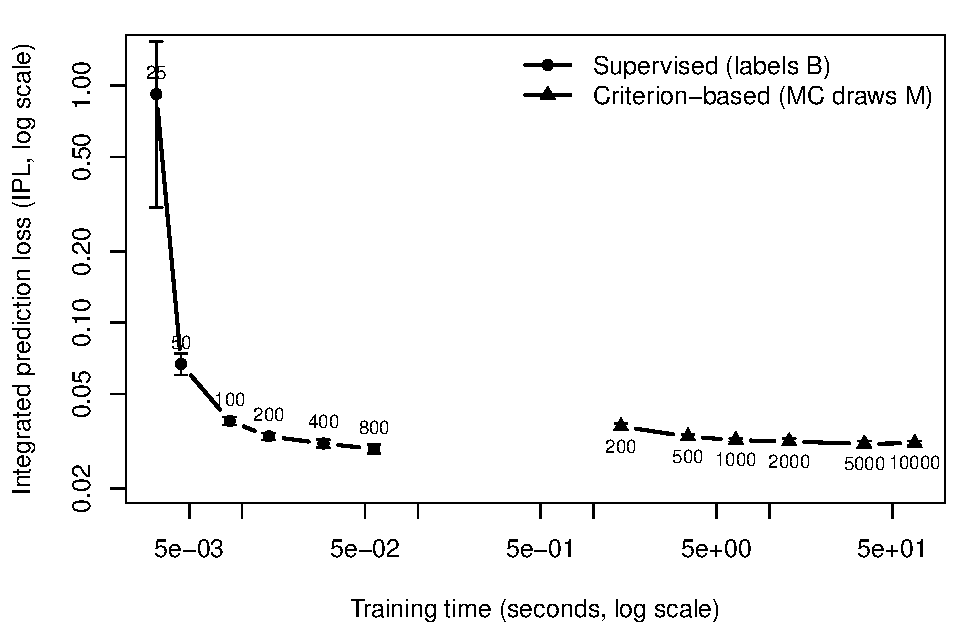
\includegraphics[width=0.85\linewidth]{toy_gms_ipl_vs_time}
\caption{Toy weighted-ridge example. Integrated prediction loss (IPL, log scale) versus training time (log scale) for supervised match-to-optimizer training (circles, labeled by number of optimizer solves $B$) and criterion-based (GMS-style) training (triangles, labeled by number of Monte Carlo draws $M$). Both methods converge to similar IPL; the criterion-based method achieves this without computing any optimizer labels, though at higher wall-clock cost in this cheap-optimizer setting (each ridge solve is closed-form). The criterion-based advantage grows when each optimizer solve is expensive.}
\label{fig:toy-gms-ipl}
\end{figure}

\begin{table}[H]
\centering
\caption{Toy weighted-ridge example: integrated prediction loss (IPL) for a linear generator trained either by supervised matching to optimizer labels ($B$ optimizer solves) or by criterion-based (GMS-style) training ($M$ Monte Carlo draws). Values are means over 12 replications with Monte Carlo standard errors in parentheses.}
\label{tab:toy-gms-ipl}
\begin{tabular}{lccc}
\hline
 & \multicolumn{3}{c}{Training budget}\\
Method & $B{=}50$ & $B{=}200$ & $B{=}800$\\
\hline
Supervised match-to-optimizer & 0.067 (0.003) & 0.033 (0.001) & 0.029 (0.001) \\
\hline
 & $M{=}500$ & $M{=}2{,}000$ & $M{=}10{,}000$\\
\hline
Criterion-based (GMS-style) & 0.033 (0.000) & 0.032 (0.000) & 0.031 (0.000) \\
\hline
\end{tabular}
\end{table}


\subsection{Extensions and connections}

The template developed above connects to several existing ideas and extends naturally to non-standard losses.

The idea of jointly updating parameters and hyper-parameters within a single iterative scheme has precedent in data augmentation methods. \citet{polson2011data} show how ECME-style updates \citep{liu1994ecme} can jointly estimate parameters $\beta$ and the regularization parameter for support vector machines. Writing $\xi$ for their regularization strength (denoted $\nu$ in their paper; we use $\xi$ here to avoid conflict with the degrees-of-freedom parameter $\nu$ used elsewhere in our paper), with $L^\alpha$ penalty and prior shape parameters $a,b$, their update for a model with $k$ nonzero coefficients and prior scales $\sigma_j$ is
\[
(\xi^{-\alpha})^{(g+1)} = \dfrac{b+\sum_{j=1}^{k}|\beta_j^{(g+1)}/\sigma_j|^{\alpha}}{a-1+k/\alpha}.
\]
In our framework, such closed-form hyper-parameter updates correspond to solving the outer problem \eqref{eq:outer} analytically when $\mathcal{C}$ has a conjugate form. More broadly, the GMS implementation of \citet{shin2024generative}, including an R package and PyTorch code, aligns directly with our inner problem \eqref{eq:inner}.

Another useful extension is the ``quantile trick'' for turning quantile-regression (check) loss into a weighted least-squares form via a variance--mean Gaussian envelope \citep{polson2016mixtures}. Here $u$ denotes an auxiliary scale variable in the envelope representation (distinct from the uniform draws used for WBB weights). For $q\in(0,1)$ and residual $r$, define the (asymmetric) absolute/hinge loss
\[
\rho_q(r) = |r| + (2q-1)r,
\]
which equals twice the standard check loss $\rho_q^{\mathrm{std}}(r) = r\,(q - \mathbf{1}_{r<0})$; the factor of two does not affect the optimizer.
\citet{polson2016mixtures} show that $\rho_q$ admits a quadratic envelope in an auxiliary variable $u>0$: the check loss equals $\inf_{u>0}$ of a quadratic form in $r$ plus a function of $u$ alone, and the conditional mode of $u$ given $r$ is
\[
\hat u(r)=\mathrm{sgn}(r)/r = 1/|r| \quad (r \neq 0);
\]
in practice one regularizes via $\hat{u}_\varepsilon(r)=1/\max(|r|,\varepsilon)$ for small $\varepsilon>0$.
This yields per-observation auxiliary weights $\tilde{w}_i=\hat u(r_i)$ and a shifted working response $z_i = y_i - (1-2q)/\tilde{w}_i$, so that the inner update becomes a weighted least-squares problem (plus the usual regularizer).
This connects to our main framework: once a difficult loss can be expressed through auxiliary variables as a weighted least-squares inner step, it fits the same computational template as WBB. Moreover, the quantile level $q$ plays the role of a tunable hyper-parameter; in the generator view one can treat $(\omega,q,\lambda)$ as inputs and learn an amortized map $(\omega,q,\lambda)\mapsto \hat{\theta}$, enabling rapid tuning over many $q$ (and $\lambda$) values. We leave this extension to future work.

\section{Empirical illustrations}

This section presents three empirical illustrations. Section~3.1 considers ridge regression, where GCV and CV provide exact benchmarks for the amortized generator. Section~3.2 applies the template to Student-$t$ degree-of-freedom estimation, a non-Gaussian setting where the profile likelihood is flat and MCMC is expensive. Section~3.3 demonstrates amortized tuning for a neural network on MNIST classification.

\subsection{Ridge regression}

As discussed in Section~2.2, ridge regression is the special case where all three components of our template are available in closed form. With hat matrix $A(\lambda) = X(X^\top X + n\lambda I)^{-1}X^\top$, the GCV criterion $V(\lambda) = n^{-1}\|y - A(\lambda)y\|^2 / (1 - n^{-1}\mathrm{tr}\{A(\lambda)\})^2$ provides an analytic outer criterion \citep{golub1979generalized}. This setting connects to modern discussions of double descent phenomena \citep{belkin2019reconciling,polson2025bayesian} and makes an ideal testbed for comparing the amortized generator against exact methods.

We simulate a ridge regression problem with $n=300$ observations, $p=80$ covariates drawn from an AR(1) design with autocorrelation $\rho=0.2$, true coefficients $\theta_0=(1,\ldots,1,0,\ldots,0)^\top$ (8 nonzero), and noise standard deviation $\sigma=1$. An independent test set of $n_{\mathrm{te}}=300$ is generated from the same distribution. We compare (i) GCV-selected $\lambda$, (ii) standard 5-fold CV, and (iii) an amortized ``generator proxy'' trained to map $\lambda$ to coefficients and thereby approximate the CV curve without repeated refits across $\lambda$. To avoid data leakage, the generator is trained separately for each fold using only that fold's training data. The generator proxy is a linear map from $(1,\log\lambda, (\log\lambda)^2)$ to $\theta$, deliberately simple to isolate the amortization idea.

Figure~\ref{fig:ridge-tuning} shows the estimated CV curves; Table~\ref{tab:ridge-tuning} reports the selected $\lambda$ and test MSE. The amortized proxy selects a comparable regularization parameter with a modest increase in test MSE, illustrating the trade-off between amortization speed and approximation accuracy due to the limited capacity of the quadratic generator. The corresponding code is in \texttt{code/experiments/ridge\_tuning\_demo.R}.

\begin{figure}[H]
\centering
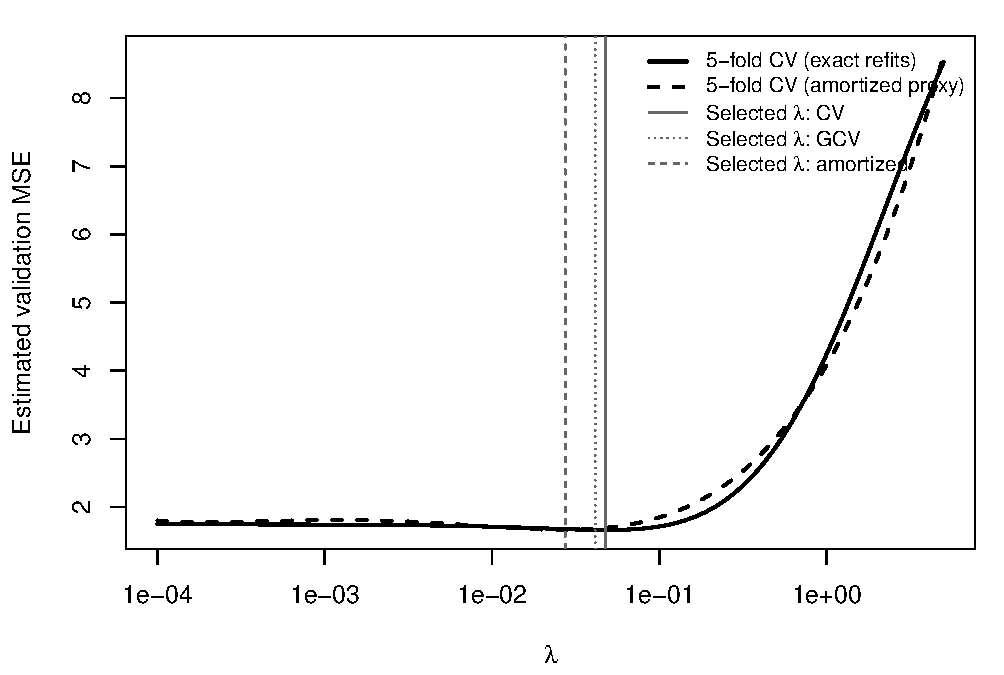
\includegraphics[width=0.85\linewidth]{ridge_tuning_demo}
\caption{Ridge tuning illustration. Solid curve: 5-fold CV requiring repeated refits for each $\lambda$. Dashed curve: amortized generator proxy. Vertical lines mark the selected $\lambda$ for each method: solid (CV), dotted (GCV), dashed (amortized proxy).}
\label{fig:ridge-tuning}
\end{figure}

\begin{table}[H]
\centering
\caption{Ridge tuning illustration (simulated data). We compare generalized cross-validation (GCV), $K$-fold cross-validation (CV), and a simple amortized generator proxy that approximates the CV curve without repeated refits across $\lambda$. Test MSE is computed on an independent hold-out test set.}
\label{tab:ridge-tuning}
\begin{tabular}{lcc}
\hline
Method & Selected $\lambda$ & Test MSE\\
\hline
GCV & 0.041 & 1.463 \\
5-fold CV & 0.047 & 1.450 \\
Amortized CV proxy (refit at selected $\lambda$) & 0.027 & 1.500 \\
\hline
\end{tabular}
\end{table}


\subsection{Student's errors}

Estimating the degrees-of-freedom parameter $\nu$ of a Student-$t$ distribution is a classical problem where standard methods encounter difficulties. The profile likelihood is flat in $\nu$ and may be strictly increasing as $\nu\to\infty$, so the MLE may not exist; improper priors on $\nu$ can lead to improper posteriors, while proper priors (e.g., exponential) may dominate the analysis \citep{fonseca2008objective}. Moreover, the marginal likelihood $p(y\mid\nu)$ is nonlinear in $\nu$, making Metropolis--Hastings proposals difficult to tune.

Consider observations $y_1,\ldots,y_n$ from a location-scale $t$-distribution. The per-observation negative log-likelihood for parameters $\theta=(\mu,\sigma)$ and fixed $\nu$ is
\[
\ell(y_i \mid \mu,\sigma,\nu) = -\log\Gamma\!\left(\tfrac{\nu+1}{2}\right) + \log\Gamma\!\left(\tfrac{\nu}{2}\right) + \tfrac{1}{2}\log(\nu\pi\sigma^2) + \tfrac{\nu+1}{2}\log\!\left(1 + \frac{(y_i-\mu)^2}{\nu\sigma^2}\right).
\]
A useful perspective is the scale-mixture-of-normals representation: $y_i \mid \tau_i \sim N(\mu, \sigma^2/\tau_i)$ with $\tau_i \sim \mathrm{Gamma}(\nu/2, \nu/2)$, which integrates to the $t_\nu(\mu,\sigma^2)$ marginal. This representation connects the $t$-distribution to the auxiliary-variable framework and makes the dependence on $\nu$ enter through the mixing distribution.

In our template, $\nu$ plays the role of the hyper-parameter $h$, and $\theta = (\mu,\sigma)$ are the model parameters. The inner problem~\eqref{eq:inner} becomes, for WBB block weights $\omega$ and fixed $\nu$,
\[
\hat\theta(\omega,\nu) = \arg\min_{(\mu,\sigma)}\; \frac{1}{n}\sum_{i=1}^n \omega_i\,\ell(y_i \mid \mu,\sigma,\nu),
\]
solved by numerical optimization. The generator $g_\varphi$ learns the map $(\omega,\nu)\mapsto (\hat\mu, \hat\sigma)$; we use a linear generator with features $(1,\nu,\nu^2,\omega_1,\ldots,\omega_K)$ (where $K=16$ is the number of WBB blocks), trained in supervised mode (A) on $B=200$ optimizer labels drawn from random $(\omega,\nu)$ pairs. The outer criterion~\eqref{eq:outer} is the validation negative log-likelihood, evaluated over a grid $\nu\in\{1.5, 2.0,\ldots, 15.0\}$:
\[
\hat\nu = \arg\min_\nu \sum_{i\in\mathcal{D}_{\mathrm{val}}} \ell\!\left(y_i \mid g_\varphi(\mathbf{1},\nu),\, \nu\right),
\]
where $g_\varphi(\mathbf{1},\nu)$ is the generator evaluated at unit weights (point estimate). Once $\hat\nu$ is selected, WBB uncertainty summaries for $(\mu,\sigma)$ are obtained by resampling: draw $\omega^{(m)}\sim\pi(\omega)$, compute $\theta^{(m)} = g_\varphi(\omega^{(m)},\hat\nu)$, and examine the empirical distribution of $\{\theta^{(m)}\}_{m=1}^M$.

We generate $n_{\mathrm{total}}=500$ observations with $\nu_{\mathrm{true}}=4$, $\mu_{\mathrm{true}}=2$, and $\sigma_{\mathrm{true}}=1.5$, split into $n_{\mathrm{train}}=350$ and $n_{\mathrm{val}}=150$. Figure~\ref{fig:t-dist} shows, for one illustrative dataset, that the generator closely tracks the profile MLE validation curve, with both methods finding the minimum near $\nu=4$.

With $n=350$ and heavy tails ($\nu=4$), the sample estimates of $\mu$ and $\sigma$ vary substantially across realizations, so a single dataset can be misleading. Figure~\ref{fig:t-dist-reps} shows the results across 20 independent replications. The location and scale estimates are centered on the true values for both methods: $\hat\mu_{\mathrm{MLE}} = 2.02\pm 0.10$, $\hat\sigma_{\mathrm{MLE}} = 1.50\pm 0.11$ versus $\hat\mu_{\mathrm{gen}} = 2.02\pm 0.10$, $\hat\sigma_{\mathrm{gen}} = 1.48\pm 0.12$ (Figure~\ref{fig:t-dist-reps}, middle and right panels). The selected $\nu$ has high variance and is upward-biased for both methods ($\hat\nu_{\mathrm{MLE}} = 5.3\pm 2.9$, $\hat\nu_{\mathrm{gen}} = 5.2\pm 2.4$; Figure~\ref{fig:t-dist-reps}, left panel), reflecting the asymmetry of the profile likelihood: steep for small $\nu$ but flat as $\nu\to\infty$ \citep{fonseca2008objective}. The average WBB posterior standard deviation is 0.089 for $\mu$ (versus cross-replicate sd of 0.10) and 0.075 for $\sigma$ (versus 0.12); the WBB is slightly under-dispersed for $\sigma$, consistent with its first-order asymptotic justification \citep{newton2021weighted}. Table~\ref{tab:t-dist-tuning} summarizes the cross-replicate results. The code is in \texttt{code/experiments/t\_dist\_tuning.R}.

\begin{figure}[H]
\centering
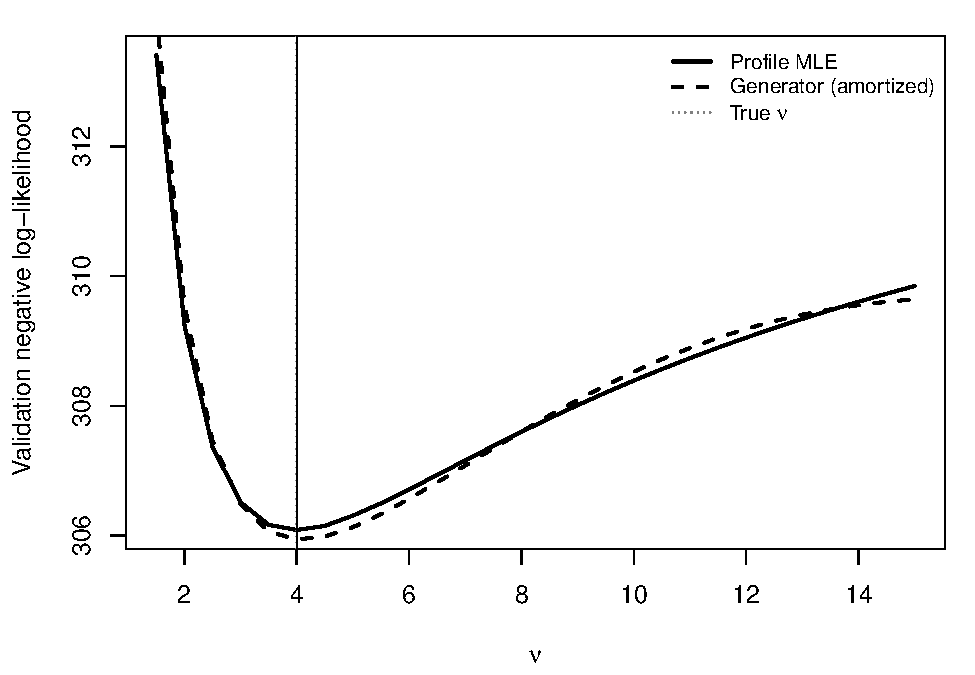
\includegraphics[width=0.65\linewidth]{t_dist_tuning}
\caption{Student-$t$ tuning, single dataset. Validation negative log-likelihood as a function of $\nu$ for profile MLE (solid) and the amortized generator (dashed); the vertical line marks the true $\nu=4$. Both methods find the minimum near $\nu=4$ on this dataset.}
\label{fig:t-dist}
\end{figure}

\begin{figure}[H]
\centering
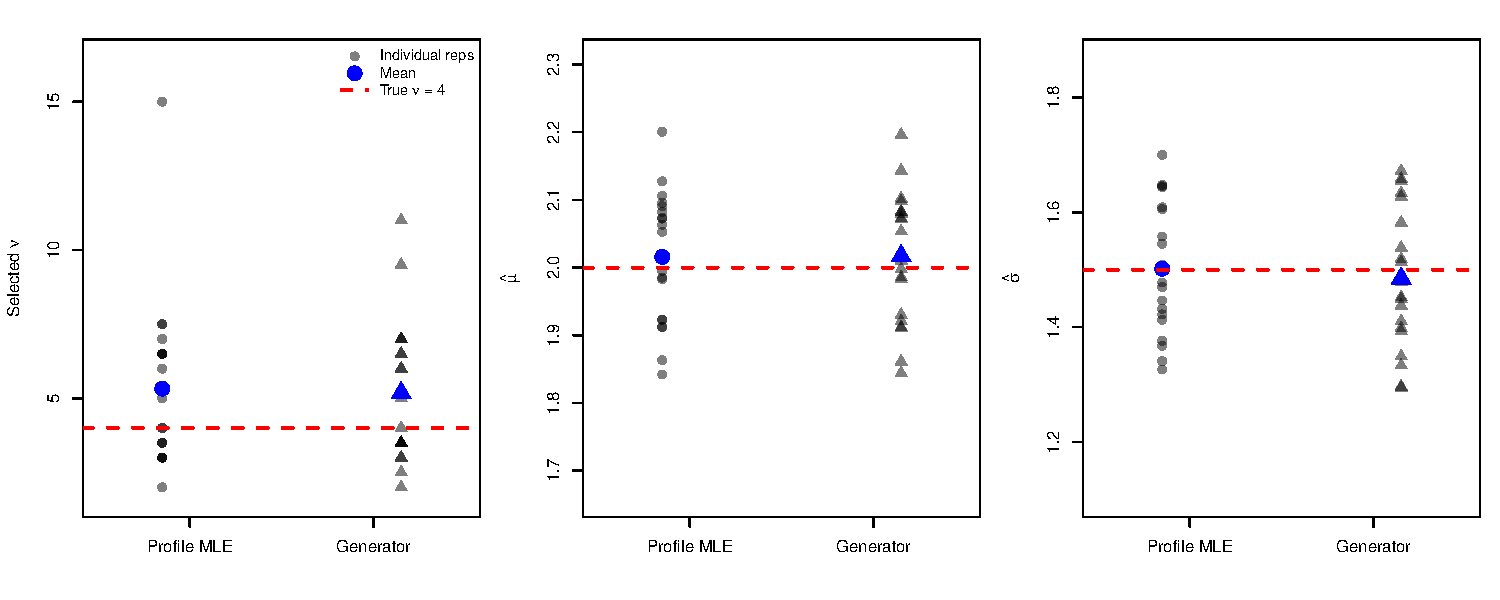
\includegraphics[width=0.95\linewidth]{t_dist_replicates}
\caption{Student-$t$ tuning, 20 replications. Each point is one independent dataset ($n=500$, $\nu_{\mathrm{true}}=4$, $\mu_{\mathrm{true}}=2$, $\sigma_{\mathrm{true}}=1.5$). Blue markers show means. Left: selected $\nu$ (upward-biased due to flat profile likelihood). Middle and right: $\hat\mu$ and $\hat\sigma$ are centered on the true values (red dashed lines) for both profile MLE and the generator.}
\label{fig:t-dist-reps}
\end{figure}

\begin{table}[H]
\centering
\caption{Student-$t$ tuning results over 20 replications ($n_{\mathrm{train}}=350$, $n_{\mathrm{val}}=150$). True parameters: $\nu=4$, $\mu=2.000$, $\sigma=1.500$. Values are means $\pm$ standard deviations across replications.}
\label{tab:t-dist-tuning}
\begin{tabular}{lccc}
\hline
Method & Selected $\nu$ & $\hat{\mu}$ & $\hat{\sigma}$ \\
\hline
Profile MLE & $5.3 \pm 2.9$ & $2.02 \pm 0.10$ & $1.50 \pm 0.11$ \\
Generator (amortized) & $5.2 \pm 2.4$ & $2.02 \pm 0.10$ & $1.48 \pm 0.12$ \\
WBB posterior mean ($\pm$ avg sd) & --- & $2.02$ ($\pm$ $0.089$) & $1.49$ ($\pm$ $0.075$) \\
\hline
\end{tabular}
\end{table}


\subsection{Deep learning}

To demonstrate the generative WBB template in a deep-learning setting, we apply it to MNIST classification. The target model is a two-layer MLP ($784\to 64\to 10$, ReLU activation, cross-entropy loss) with $50{,}890$ parameters. The generator (hyper-network) is a three-layer MLP (hidden dimension 128) that maps a $(1+K)$-dimensional input --- a normalized $\log_{10}\lambda$ concatenated with $K=16$ block bootstrap weights $\omega$ --- to the full parameter vector $\theta$. Training uses the criterion-based objective (mode~B) over 5 epochs with Adam (learning rate $10^{-3}$, batch size 128), minimizing the WBB-weighted data loss plus $\lambda\|\theta\|_2^2$ penalty across a range $\lambda \in [10^{-5}, 10^{-1}]$. The 60{,}000 MNIST training images are split into 50{,}000 for training and 10{,}000 for validation; the standard 10{,}000-image test set is used only for final evaluation. Hyper-parameter selection (choosing $\lambda$) is based on validation accuracy, not the test set.

Figure~\ref{fig:mnist-tuning} shows the validation loss and accuracy paths produced by the generator with unit weights ($\omega=\mathbf{1}$); Table~\ref{tab:mnist-tuning} reports representative performance metrics for one run. Because the generator accepts bootstrap weights $\omega$ as input, it also produces WBB uncertainty summaries: resampling $\omega$ from a Dirichlet distribution at the selected $\lambda$ yields a distribution of fitted models whose spread provides an uncertainty estimate. The baseline model is trained with explicit $L_2$ regularization matching the generator's penalty.

Over 20 independent replications (Figure~\ref{fig:mnist-reps}), the generator achieves test accuracy $95.3\%\pm 0.5\%$ (mean $\pm$ sd) versus $96.7\%\pm 0.2\%$ for the baseline trained from scratch. The accuracy gap is consistent across seeds. The WBB posterior mean accuracy is $95.2\%\pm 0.5\%$ with average posterior standard deviation $0.12\%$. Evaluating the full 20-point $\lambda$ tuning curve takes approximately $28$s per run on CPU, compared to $35$s to train a single baseline model.

\begin{figure}[H]
\centering
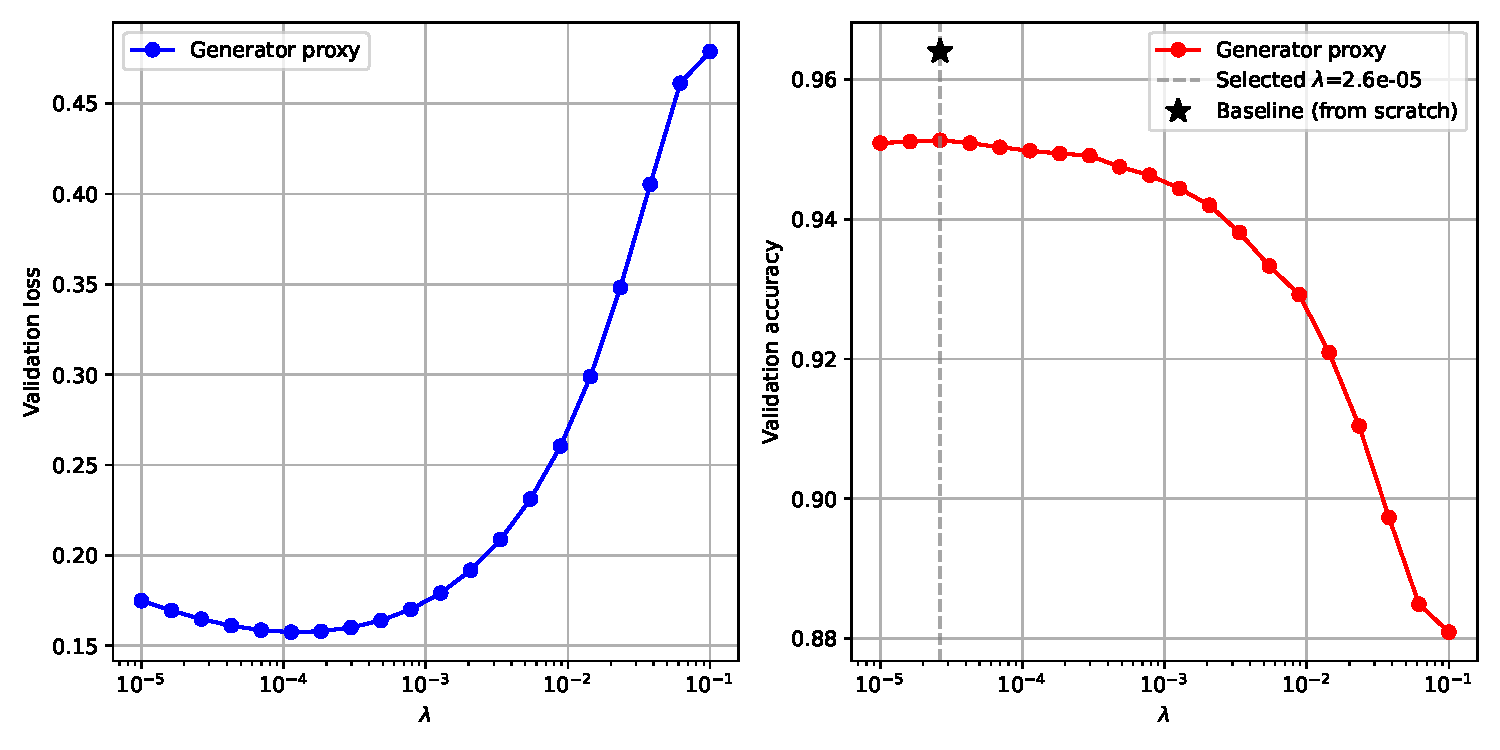
\includegraphics[width=0.85\linewidth]{mnist_generator_tuning}
\caption{MNIST tuning illustration. Left: validation loss; right: validation accuracy as functions of $\lambda$, both produced by a single forward pass through the generator (with unit weights $\omega=\mathbf{1}$) for each $\lambda$ value. The star marks the baseline model trained from scratch at the generator-selected $\lambda$.}
\label{fig:mnist-tuning}
\end{figure}

\begin{table}[H]
\centering
\caption{MNIST results for one illustrative run. Top rows: validation-set performance of the generator across $\lambda$ values. Bottom rows: test-set accuracy at the selected $\lambda$ for the generator (point estimate with $\omega=\mathbf{1}$), baseline (trained from scratch with matching $L_2$ penalty), and WBB posterior mean ($\pm$ standard deviation over 50 bootstrap weight draws). Cross-replicate statistics over 20 independent runs are reported in the text.}
\label{tab:mnist-tuning}
\begin{tabular}{ccc}
\hline
$\lambda$ & Val.~Loss & Val.~Acc. \\
\hline
1.0e-05 & 0.1749 & 0.9509 \\
1.1e-04 & 0.1575 & 0.9498 \\
1.3e-03 & 0.1792 & 0.9444 \\
1.4e-02 & 0.2989 & 0.9209 \\
1.0e-01 & 0.4788 & 0.8809 \\
\hline
Selected ($\lambda=2.6e-05$), test & - & 0.9565 \\
Baseline ($\lambda=2.6e-05$), test & - & 0.9670 \\
WBB posterior mean, test & - & 0.9562 $\pm$ 0.0008 \\
\hline
\end{tabular}

\end{table}

\begin{figure}[H]
\centering
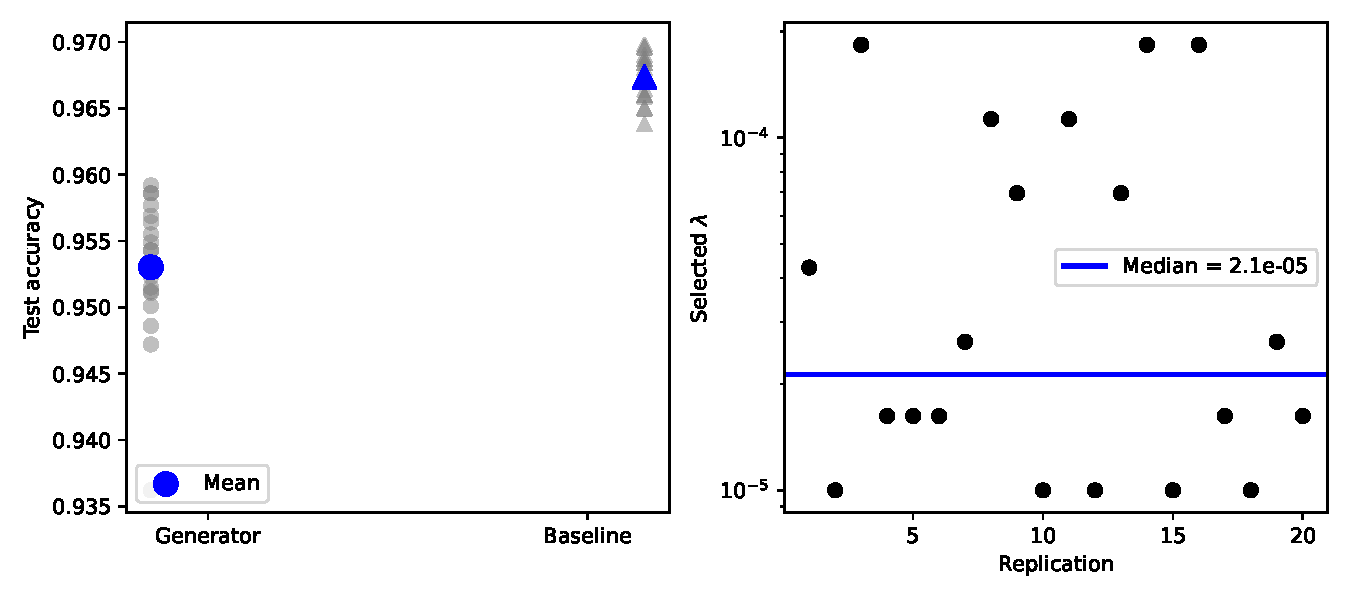
\includegraphics[width=0.85\linewidth]{mnist_replicates}
\caption{MNIST tuning, 20 replications. Left: test accuracy for the generator (circles) and baseline (triangles) across independent runs; blue markers show means. The accuracy gap (${\approx}\,1.4$ percentage points) is stable across seeds. Right: selected $\lambda$ varies across runs (log scale) with median $2.1\times 10^{-5}$.}
\label{fig:mnist-reps}
\end{figure}

\section{Discussion}

This paper develops a unified view of hyper-parameter tuning as an outer criterion evaluated under an induced (possibly randomized) inner optimization map, and highlights amortization via generators/transport maps as a way to make repeated tuning and uncertainty summaries computationally feasible. By connecting GCV, the weighted Bayesian bootstrap (WBB), and GMS-style criterion-based training, we provide a coherent framework for scalable hyper-parameter learning.

The central benefit of the proposed approach is the amortization of the optimization cost. Once trained, the generator produces fitted parameters for any new hyper-parameter value via a single forward pass, replacing the expensive retraining loop. This speedup is particularly valuable for exploratory analysis and naturally extends to high-dimensional tuning, where the generator can accept vectors of hyper-parameters (e.g., layer-specific penalties, dropout rates) to explore spaces where grid search is infeasible. Because the generator also accepts WBB bootstrap weights as input, it simultaneously provides posterior uncertainty summaries by resampling these weights at test time, as demonstrated in both the Student-$t$ and MNIST experiments.

Our ridge regression experiment illustrated a key trade-off: a simple generator (linear or quadratic map) approximates the tuning curve well but may sacrifice some accuracy relative to exact refitting. The Student-$t$ experiment shows that even a linear generator accurately tracks the profile likelihood for a non-Gaussian model, and that WBB posterior draws provide reasonable uncertainty summaries centered near the true parameters. In deep learning, the generator must have sufficient capacity relative to the complexity of the hyper-parameter-to-parameter map; the MNIST experiment shows that a modest neural generator recovers most of the baseline accuracy while enabling rapid tuning-curve exploration.

Compared to gradient-based hyperparameter optimization \citep{maclaurin2015gradient} and bilevel approaches \citep{franceschi2018bilevel}, which also avoid retraining loops by differentiating through the training procedure, the generator approach has a distinct advantage: it produces an explicit map from hyper-parameters to parameters that can be queried at arbitrary $h$ values without backpropagating through training. The trade-off is that the generator must be trained, and its accuracy depends on having sufficient capacity.

Several caveats deserve mention. The generator itself must be trained, which is a one-time upfront cost; the approach is most attractive when many tuning evaluations or repeated uncertainty summaries are needed. The WBB posterior-approximation property on which the uncertainty summaries rest is a conjecture \citep{newton2021weighted}, supported by asymptotic arguments and empirical evidence but not yet a theorem; our Student-$t$ experiments show that the WBB posterior is slightly under-dispersed relative to frequentist variability, consistent with its first-order justification. In the MNIST experiment, the generator achieves approximately 95\% test accuracy versus 97\% for the baseline trained from scratch --- a gap that reflects the finite capacity of the generator rather than a limitation of the tuning framework itself.

The number of WBB blocks $K$ (16 in our experiments) is a tunable setting whose effect on posterior quality we have not studied; investigating this sensitivity is left for future work. Several other avenues for future work remain. First, adaptive sampling strategies for $(\lambda, \omega)$ during generator training could focus computational effort on the most relevant regions of hyper-parameter space. Second, architectural choices for the generator (e.g., rank-1 modulations, LoRA-style adapters) could further reduce the overhead of training the transport map. Finally, extending this framework to non-differentiable hyper-parameters (e.g., architecture search) remains an open direction.

\bibliography{HyperTuning}

\appendix
\section{Algorithm}

\begin{algorithm}[H]
\caption{Generative WBB for hyper-parameter tuning and uncertainty summaries}
\label{alg:gwbb}
\begin{algorithmic}[1]
\Require Training data $\mathcal{D}_{\mathrm{train}}$, validation data $\mathcal{D}_{\mathrm{val}}$; hyper-parameter proposal $\Pi(\lambda,\eta)$; weight distribution $\pi(\omega)$; samples $B$ (training) and $M$ (evaluation); generator family $g_{\varphi}$.
\State \textbf{(Choose generator training mode)} Either (A) supervised regression to match $\hat{\theta}$, or (B) criterion-based training (as in GMS).
\State \textbf{(Training draws)} For $b=1,\ldots,B$:
\State \hspace{1em}Sample $(\lambda^{(b)},\eta^{(b)})\sim \Pi(\lambda,\eta)$ and weights $\omega^{(b)}\sim \pi(\omega)$.
\If{mode (A)}
\State \hspace{1em}Compute $\hat{\theta}^{(b)} \approx \arg\min_{\theta}\Big\{\frac{1}{n}\sum_{i=1}^n \omega_i^{(b)}\,\ell_{\eta^{(b)}}(y_i\mid \theta) + \lambda^{(b)}\phi(\theta)\Big\}$ using SGD on $\mathcal{D}_{\mathrm{train}}$ (reweighted mini-batches).
\State \textbf{(Train generator)} Fit $\hat{\varphi}\in\arg\min_{\varphi}\sum_{b=1}^B \big\|\hat{\theta}^{(b)} - g_{\varphi}(\omega^{(b)},\lambda^{(b)},\eta^{(b)})\big\|^2$.
\Else
\State \textbf{(Train generator)} Fit $\hat{\varphi}\in\arg\min_{\varphi}\sum_{b=1}^B \Big[\frac{1}{n}\sum_{i=1}^n \omega_i^{(b)}\,\ell_{\eta^{(b)}}(y_i\mid g_{\varphi}(\omega^{(b)},\lambda^{(b)},\eta^{(b)})) + \lambda^{(b)}\phi\big(g_{\varphi}(\omega^{(b)},\lambda^{(b)},\eta^{(b)})\big)\Big]$.
\EndIf
\State \textbf{(Tune hyper-parameters)} For candidate $(\lambda,\eta)$:
\State \hspace{1em}Estimate $J(\lambda,\eta)\approx \frac{1}{M}\sum_{m=1}^M \mathcal{R}(g_{\hat{\varphi}}(\omega^{(m)},\lambda,\eta);\mathcal{D}_{\mathrm{val}})$ with $\omega^{(m)}\sim\pi(\omega)$, and set $(\hat{\lambda},\hat{\eta})\in\arg\min_{\lambda,\eta} J(\lambda,\eta)$.
\State \textbf{(Uncertainty summaries)} With tuned $(\hat{\lambda},\hat{\eta})$, sample $\omega^{(m)}\sim\pi(\omega)$, set $\theta^{(m)}=g_{\hat{\varphi}}(\omega^{(m)},\hat{\lambda},\hat{\eta})$, and summarize predictive uncertainty using the empirical distribution of $\{p(y\mid x,\theta^{(m)})\}_{m=1}^M$.
\end{algorithmic}
\end{algorithm}

\end{document}